%%% Exemplo de utilização da classe ITA
%%%
%%%   por        Fábio Fagundes Silveira   -  ffs [at] ita [dot] br
%%%              Benedito C. O. Maciel     -  bcmaciel [at] ita [dot] br
%%%              Giovani Volnei Meinertz   -  giovani [at] ita [dot] br
%%%    	         Hudson Alberto Bode       -  bode [at] ita [dot]br
%%%    	         P. I. Braga de Queiroz    -  pi [at] ita [dot] br
%%%    	         Jorge A. B. Gripp         -  gripp [at] ita [dot] br
%%%    	         Juliano Monte-Mor         -  jamontemor [at] yahoo [dot] com [dot] br
%%%    	         Tarcisio A. B. Gripp      -  tarcisio.gripp [at] gmail [dot] com
%%%
%%%   Versão para overleaf:
%%%   por        Alejandro A. Rios Cruz    - aarc.88@gmail.com
%%%              Saulo Gómez               - sagomezs@unal.edu.co
%%%              Ocimar Santos             - ocimar.acad@gmail.com
%%%
%%%   Template disponibilizado em:
%%%              Overleaf: https://pt.overleaf.com/latex/templates/thesis-template-aeronautics-institute-of-technology-ita/yhfrqqydpygk
%%%
%%%   Contribuia você também!
%%%              GitHub:   https://github.com/AlejandroRios/Template_Thesis_ITA
%%%
%%%  IMPORTANTE: O texto contido neste exemplo nao significa absolutamente nada.  :-)
%%%              O intuito aqui eh demonstrar os comandos criados na classe e suas
%%%              respectivas utilizacoes.
%%%
%%%  Tese.tex  2016-08-25
%%%  $HeadURL: http://www.apgita.org.br/apgita/teses-e-latex.php $
%%%
%%% ITALUS
%%% Instituto Tecnológico de Aeronáutica --- ITA, Sao Jose dos Campos, Brasil
%%%                   http://groups.yahoo.com/group/italus/
%%% Discussion list: italus {at} yahoogroups.com
%%%
%++++++++++++++++++++++++++++++++++++++++++++++++++++++++++++++++++++++++++++++
% Para alterar o TIPO DE DOCUMENTO, preencher a linha abaixo \documentclass[?]{?}
%   \documentclass[tg]{ita}			= Trabalho de Graduacao
%   \documentclass[tgfem]{ita}	= Para Engenheiras
%   								msc     		= Dissertacao de Mestrado
%   								mscfem   		= Para Mestras
%   								dsc      		= Tese de Doutorado
%   								dscfem   		= Para Doutoras
%   								quali    		= Exame de Qualificacao
%   								qualifem 		= Exame de Qualificacao para Doutoras
% Para 'Draft Version'/'Versao Preliminar' com data no rodape, adicionar 'dv':
%   \documentclass[dsc, dv]{ita}
% Para trabalhos em Inglês, adicionar 'eng':
%   \documentclass[dsc, eng]{ita}
%		\documentclass[dsc, eng, dv]{ita}
%++++++++++++++++++++++++++++++++++++++++++++++++++++++++++++++++++++++++++++++
\documentclass[tg]{ita}    % ITA.cls based on standard book.cls
% Quando alterar a classe, por exemplo de [msc] para [msc, eng]) rode mais uma vez o botão BUILD OUTPUT caso haja erro
\usepackage{ae}
\usepackage{graphicx}
\usepackage{epsfig}
\usepackage{amsmath}
\usepackage{amssymb}
\usepackage{subfig}
\usepackage{multirow}
\usepackage{float}
\usepackage{amsthm}
\usepackage{url}         % formats URL addresses properly
\usepackage{appendix}    % allows appendix section to be included
\usepackage{lscape}      % allows a page to be rendered in landscape mode
\usepackage{multicol}    % allows text in multi columns
\usepackage{cancel}      % needed to show canceled terms in equations
\usepackage{lettrine}
\usepackage{float}
\usepackage{placeins}


%HHHHHHHHHHHHHHHHHHHHHHHHHHHHHHHHHHHHHHHHHHHHHHHHHHHHHHHHHHHHHHHHHHHHHHHHHHHHHHHHHHHHHHHHHHHHHHHHHHHHHHHHHHHH
%\usepackage{subfigure}
%\usepackage{subfigmat}
%PACOTEFIGURAS_SE _ERRADO_ESXCLUIR_ACIMA
\usepackage{booktabs}
%PACOTETABELAS_SE _ERRADO_ESXCLUIR_ACIMA
%HHHHHHHHHHHHHHHHHHHHHHHHHHHHHHHHHHHHHHHHHHHHHHHHHHHHHHHHHHHHHHHHHHHHHHHHHHHHHHHHHHHHHHHHHHHHHHHHHHHHHHHHHHHH

%++++++++++++++++++++++++++++++++++++++++++++++++++++++++++++++++++++++++++++++
% Espaçamento padrão de todo o documento
%++++++++++++++++++++++++++++++++++++++++++++++++++++++++++++++++++++++++++++++
\onehalfspacing

%singlespacing Para um espaçamento simples
%onehalfspacing Para um espaçamento de 1,5
%doublespacing Para um espaçamento duplo

%++++++++++++++++++++++++++++++++++++++++++++++++++++++++++++++++++++++++++++++
% Identificacoes (se o trabalho for em inglês, insira os dados em inglês)
% Para entradas abreviadas de Professora (Profa.) em português escreva: Prof$^\textnormal{a}$.
%++++++++++++++++++++++++++++++++++++++++++++++++++++++++++++++++++++++++++++++
\course{Engenheria Aeroespacial}  % Programa de PG ou Curso de Graduação
%\area{Aircraft Design} % Área de concentração na PG (Não utilizado no caso de TG)

% Autor do trabalho: Nome Sobrenome
\authorgender{masc}                     %sexo: masc ou fem
\author{Pedro Kuntz}{Puglia}
\itaauthoraddress{Rua H8C, Ap. 303}{12.228- 462}{São José dos Campos- SP}

% Titulo da Tese/Dissertação
\title{Caracterização de sistema de propulsão a gás frio com empuxo vetorial}

% Orientador
\advisorgender{masc}                    % masc ou fem
\advisor{Prof.~Dr.}{Leonardo Gouvêa}{ITA}

% Coorientador (Caso não haja coorientador, colocar ambas as variáveis \coadvisorgender e \coadvisor comentadas, com um % na frente)
% \coadvisorgender{fem}									% masc ou fem
% \coadvisor{Prof$^\textnormal{a}$.~Dr$^\textnormal{a}$.}{Doralice Serra}{OVNI}

% Pró-reitor da Pós-graduação
% \bossgender{masc}												% masc ou fem
% \boss{Prof.~Dr.}{John von Neumann}

%Coordenador do curso no caso de TG
\bosscoursegender{fem}									% masc ou fem
\bosscourse{Profa.~Dra.}{Cristiane Martins}

% Palavras-Chaves informadas pela Biblioteca -> utilizada na CIP
\kwcip{Propulsão}
\kwcip{Empuxo Vetorial}
\kwcip{Gás Frio}

% membros da banca examinadora

% \examiner{Prof. Dr.}{Alan Turing}{Presidente}{ITA}
% \examiner{Prof. Dr.}{Linus Torwald}{}{UXXX}
% \examiner{Prof. Dr.}{Richard Stallman}{}{UYYY}
% \examiner{Prof. Dr.}{Donald Duck}{}{DYSNEY}
% \examiner{Prof. Dr.}{Mickey Mouse}{}{DISNEY}

% Data da defesa (mês em maiúsculo, se trabalho em inglês, e minúsculo se trabalho em português)
\date{23}{novembro}{2022}

% Número CDU - (somente para TG)
\cdu{???.??}

% Glossario
\makeglossary
\frontmatter

\begin{document}
%%%%%%%%%%%%%%%%%%%%%%%%%%%%%%%%%%%%%%%%%
%%% - - Modelo para relatório ITA - - %%%
%%%%%%%%%%%%%%%%%%%%%%%%%%%%%%%%%%%%%%%%%
%%%    Documente as mudanças e os     %%%
%%%       upgrades na estrutura       %%%
%%%%%%%%%%%%%%%%%%%%%%%%%%%%%%%%%%%%%%%%%

\documentclass[12pt, a4paper]{article}

% Fonte e símbolos
% \usepackage{fontspec}
% \setmainfont{Times New Roman}
\usepackage[brazilian]{babel}
% Tamanho padrão da folha
\usepackage[left=1.5cm,right=1.5cm,top=1.5cm,bottom=1.5cm]{geometry}
\usepackage{csquotes}
\usepackage{latexsym}
\usepackage{amsmath}
\usepackage{textcomp}
\usepackage{gensymb}
\usepackage{indentfirst}
\usepackage{amssymb}
\usepackage{graphicx}
\usepackage{pbox}
\usepackage[dvipsnames]{xcolor}
\usepackage{float}
\usepackage{verbatim}
\usepackage{adjustbox}


% Top, mid e bottomrule para tabelas
\usepackage{booktabs}
\usepackage{multirow}

% Gerenciamento de referências
% É possível adicionar "style=abnt"
\usepackage[
backend=biber,
sorting=none,
style=abnt-numeric
]{biblatex}
\addbibresource{references.bib}

% Tamanho 12 para os títulos de seção e subsseção
\usepackage[tiny]{titlesec}

% Package para fazer referências no corpo do texto
\usepackage{hyperref}

% Packages para uso de subfigure
\usepackage{caption}
\usepackage{subcaption}
\usepackage{ragged2e}

\begin{document}

\begin{titlepage}
\begin{center}

\begin{figure}
\begin{center}

\includegraphics[width=9cm]{Images/ita-logo.png}
\end{center}
\end{figure}

\begin{huge}
\bf{\sc{Instituto Tecnológico de Aeronáutica}} \\
\vspace*{0.15in}
\end{huge}

\begin{Large}
\bf{\sc{Divisão de Engenharia Aeronáutica e Aeroespacial}}\\
\end{Large}

\begin{Large}
\vspace*{0.2in}
\textbf{Departamento de Eletrônica (IEE)} \\
\textbf{Projeto de ELE-27} \\

\vfill

\textbf{CubeSat}
\end{Large}

\vfill


\begin{large}
    \begin{FlushLeft}
        \textbf{Professor} \\
        Tertuliano Ribeiro Pinto \\
    \end{FlushLeft}
\end{large}

\begin{large}

\begin{FlushLeft}
    \textbf{Alunos} \\
    Ana Beatriz da Silva Machado\\
    Caio Jansen Accioly\\
    Lucas Ramalho Rocha\\
    Luísa Dallmann\\
    Mahmud Mohamad Hussein Ali Neto\\
    Mateus Silva Borges\\
    Natan Campistano de Mello\\
    Pedro Kuntz Puglia \\
\end{FlushLeft}

\end{large}
\vspace*{0.1in}
\Large{2023}
\end{center}
\end{titlepage}




\input{Tex/0.Sumário.tex}

\input{Tex/9.Referências.tex}

\end{document}

\mainmatter
% Os capitulos comecam aqui

\chapter{Introdução}
\section{Objetivo}
O objetivo deste projeto de mestrado é desenvolver técnicas de controle subótimo das juntas passivas (não atuadas) de um robô subatuado, incluindo o estudo teórico do tema, proposição de um método de controle e sua verificação
experimental em um manipulador de três graus de liberdade \cite{Nascimento1970}.

O teste \cite{Patagonios2001} e validação das técnicas de controle propostas foram realizados em um ambiente de simulação e no manipulador
experimental, adquirido através do projeto FAPESP $N^{\circ}$ 98/00649-5, que se encontra em funcionamento no Laboratório de Sistemas Inteligentes (LASI) do Departamento de Engenharia Elétrica da USP em São Carlos. De acordo com \citeonline{Furmento1995}, pode-se listar:
\begin{itemize}
\item Isso;
\item Aquilo; e
\item Aquele outro.
\end{itemize}

\section{Motivação}
Manipuladores mecânicos \cite{Sbornian2002} vêm sendo utilizados há várias décadas para a automação de tarefas
repetitivas em ambientes industriais, ambientes estes de fácil acesso tanto em termos físicos quanto em termos de baixo
risco à saúde humana. Nos últimos anos, verifica-se uma utilização cada vez maior de manipuladores em
ambientes de difícil acesso ou inóspitos, como no interior de usinas nucleares, no fundo dos oceanos e no
espaço. A localização dos manipuladores nesta nova gama de aplicações faz com que sua manutenção,
Dpós uma falha mecânica ou elétrica, seja custosa e demorada, portanto estes mecanismos requerem sofisticadas
metodologias de controle tolerante a falhas \cite{ITALUS2004}.

Após a ocorrência de uma falha em um de seus atuadores, o manipulador torna-se um sistema subatuado. Um sistema também pode se tornar subatuado quando é projetado  dessa maneira, ou quando o operador deliberadamente mantém um ou mais atuadores disponíveis inoperantes durante uma tarefa. Reduzindo o número de atuadores sem reduzir o número de graus de
liberdade e ajustando-se o sistema de controle adequado, pode-se obter um mecanismo cujo consumo de energia é menor, mas cujas propriedades são mantidas \cite{Arystides1994}.

\begin{figure}[ht]
\centering
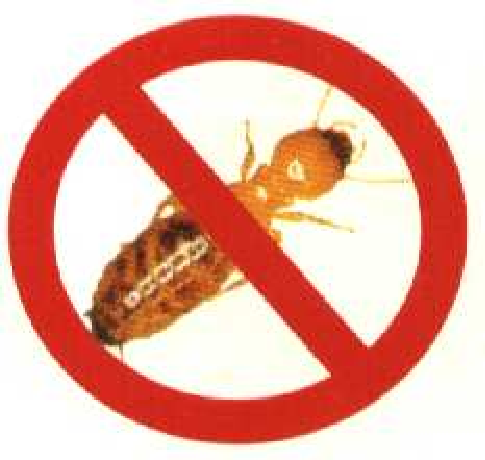
\includegraphics[width=0.5\textwidth]{Cap1/cupim}
\caption{Proibido estacionar cupins. Legenda grande, com o objetivo de demonstrar a indentação na lista de figuras.}
\label{cupim}
\end{figure}

Controle do manipulador após uma falha é fundamental do ponto de vista de operação, principalmente nos casos descritos acima, em que a localização do manipulador impede sua manutenção de forma fácil. Recentemente tem havido a combinação
de algorítmos de detecção e isolação de falhas com os de controle pós-falha em um método unificado. Uma extensão desse trabalho, que vê o problema de controle tolerante a falhas através de uma perspectiva integrada, foi proposta por
{marcel4}. Os autores apresentam um ambiente híbrido consistindo de três unidades básicas que garantem a compleição de tarefas na presença de qualquer número de juntas falhas (Figura \ref{cupim}). A primeira unidade é um esquema de detecção
e isolação de falhas que continuamente monitora o manipulador para detectar e identificar possíveis falhas nas juntas. A segunda unidade é responsável pela reconfiguração do controle. A terceira unidade é composta de algorítmos de
controle apropriados para cada tipo de configuração do robô, baseado na informação da unidade de reconfiguração \cite{COFFEE2000}.

No presente trabalho nos concentramos na unidade de algorítmo de controle, e mais especificamente no problema de controle da posição  angular de uma junta falha para qualquer posição desejada de uma maneira subótima, quando dispomos
de redundância de atuação para a realização dessa tarefa. O termo subótimo se deve ao fato de que não há garantias de otimalidade em vista das não-linearidades inerentes ao sistema e de outros fatores que serão abordados nos capítulos posteriores. Ao longo do texto, para simplificação, usaremos tanto o termo subótimo como ótimo para nos referirmos à metodologia utilizada.

Segundo, o critério de otimização utilizado será o acoplamento entre as juntas do
manipulador e neste caso, temos um sistema redundante quando ocorre falha de uma das juntas do manipulador de três juntas, e seu posicionamento é controlado pelas duas restantes. Nossa solução para o problema é baseada na formulação
de redundância local, extensivamente estudada no contexto de cinemática inversa ({nakamura}). A principal contribuição deste trabalho é a extensão deste método usando as equações dinâmicas de manipuladores subatuados e a utilização do índice de acoplamento como um critério para a minimização do torque e da energia gasta pelo sistema durante o controle das juntas falhas.

\begin{figure}[ht!]
\centering
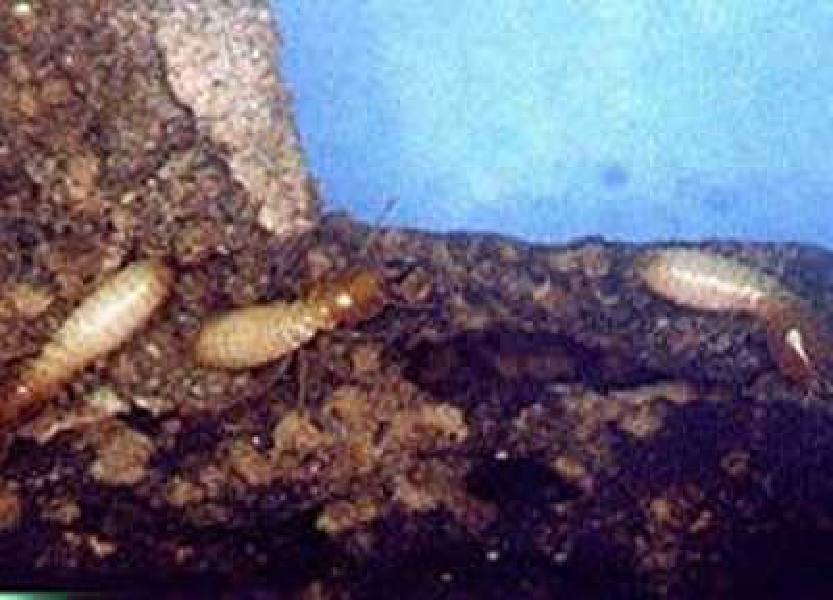
\includegraphics[width=1\textwidth]{Cap1/cupimconcreto}
\caption{Exemplo real de cupim frente ao seu dilema.}
\label{FDII}
\end{figure}

\section{Organização do trabalho}
\subsection{Sub-organização}
O capítulo 1 contém a introdução do trabalho, onde são expostos o objetivo, a motivação do mesmo, a descrição do sistema e a formulação do problema com a nomenclatura utilizada; além de uma revisão bibliográfica da literatura relacionada ao tema do trabalho.

\subsubsection{SubSub-organização}

No capítulo 2 apresentamos a modelagem dinâmica de um manipulador subatuado e o conceito de índice de acoplamento para medir o acoplamento dinâmico entre as juntas ativas e passivas. Este índice é utilizado para a análise e projeto de uma metodologia de controle subótimo do manipulador.

\subsubsection{Outra subsub-organizacao}

O capítulo 3 apresenta o controle subótimo de manipuladores através de redundância de atuação. Descreve-se a técnica de controle ponto a ponto de manipuladores subatuados. A seguir mostramos  a linearização destes por realimentação, cujo efeito é linearizar e desacoplar o sistema não linear. Finalmente é proposta uma sequência de controle subótimo local das juntas passivas visando a minimização de certos critérios como torque, velocidade e em particular a energia consumida pelo sistema. Este é de fato o tema principal deste mestrado.

É também apresentado no capítulo 4 um resumo do projeto de controladores  $H_{2}$ e $H_{\infty}$, cuja principal vantagem é a robustez na presença de incertezas paramétricas e distúrbios externos.

O capítulo 5 mostra as características e a operação do robô e do ambiente de simulação utilizados nos testes e experimentação da metodologia apresentada.

Os procedimentos da metodologia e os resultados obtidos para algumas configurações e diferentes controladores encontram-se no capítulo 6.

No capítulo 7 são apresentadas as conclusões do trabalho.

Quatro apêndices fazem parte do trabalho. O apêndice A apresenta alguns tópicos de álgebra linear que são a base do método proposto. No apêndice B são mostradas as equações da matriz de inércia e do vetor de torques não-inerciais
utilizados na modelagem dinâmica do manipulador. No apêndice C temos as expressões literais dessas equações feitas no software MAPLE e no apêndice D alguns programas feitos no software MATLAB utilizados no projeto \cite{Furmento1995}\cite{Morgado2003}.



\chapter{Modelagem Dinâmica de Cupins Cibernéticos}
\section{Modelagem no espaço das juntas}
Manipuladores subatuados diferem dos totalmente atuados pois são equipados com um número de atuadores que é sempre menor que o número de graus de liberdade (GDL). Portanto, nem todos os GDL podem ser controlados ativamente ao mesmo tempo \cite{Sbornian2004}. Por exemplo, com um manipulador planar de 3 juntas equipado com dois atuadores, ou seja, duas juntas ativas e
uma passiva, pode-se controlar ao mesmo tempo duas das juntas a qualquer instante, mas não todas. Para controlar todas as juntas de um manipulador subatuado, deve-se usar um controle sequencial. Este princípio foi provado pela primeira vez por {arai} usando  argumentos dinâmicos linearizados \cite{Joea2003}, e é a base para a modelagem no espaço das juntas e no espaço Cartesiano. A Tabela \ref{minhatab} apresenta os resultados \cite{Assenmacher1993,Silberschatz1991,Caromel1998}.

\begin{table}
\caption{Exemplo de uma Tabela}
\label{minhatab}

\center
\begin{tabular}{cccc}
  % after \\: \hline or \cline{col1-col2} \cline{col3-col4} ...
  \hline
	Parâmetro & Unidade & Valor da simulação & Valor experimental   \\
	\hline
  Comprimento, $\alpha$ & $m$ &  $8,23$  & $8,54$ \\
  Altura, $\beta$ & $m$     &  $29,1$ & $28,3$\\
	Velocidade, $v$ & $m/s$  &  $60,2$ & $67,3$\\
	\hline
\end{tabular}
\end{table}

Devido ao fato de que no máximo $n_{a}$ coordenadas generalizadas (ângulos das juntas ou variáveis cartesianas) podem ser controladas num dado instante, o vetor de coordenadas generalizadas é dividido em duas partes, representando as coordenadas generalizadas ativas e as coordenadas generalizadas passivas \cite{Callaghan1995}.

\begin{figure}[ht]
\centering
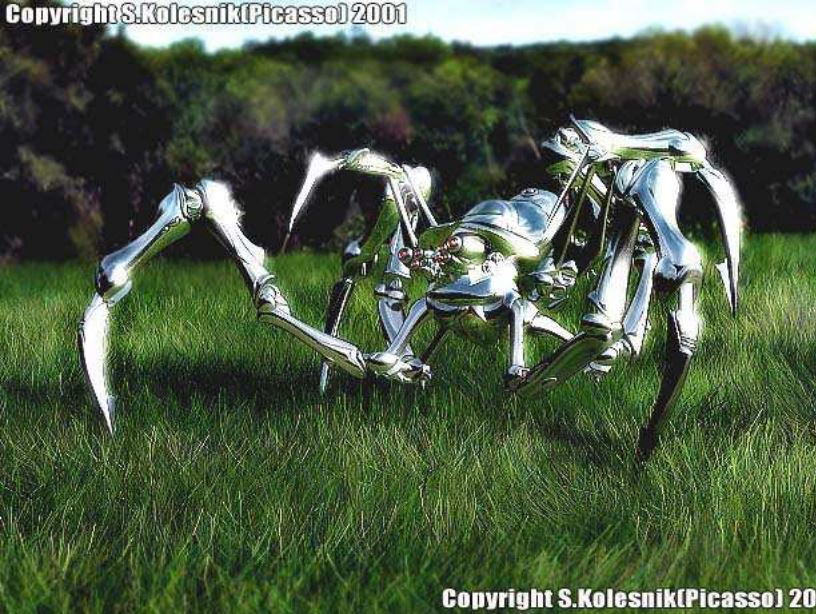
\includegraphics[width=0.75\textwidth]{Cap2/spiderrobot}
\caption{Cupim cibernético.}\label{FDIII}
\end{figure}

Considerando um robô manipulador rígido, malha aberta, e de $n$-juntas em série. Seja $q$ a representação de seu vetor de posição angular das juntas  e $\tau$ a representação de seu vetor de torque. A equação dinâmica pelo método de
Lagrange é dada por:
\begin{equation} \label{eq:lagr1}
\frac{d}{dt}(\frac{\partial L}{\partial \dot{q}})-\frac{\partial L}{\partial q}=\tau^{T}.
\end{equation}
O Lagrangiano $L$ é definido como a diferença entre as energias cinética e potencial do sistema:
\begin{equation} \label{L}
L=T-P
\end{equation}

A energia cinética total dos ligamentos é representada:
\begin{equation} \label{energT}
T=\frac{1}{2}\dot{q}^{T}M(q)\dot{q}
\end{equation}


\chapter{Controle Robusto de Concretos Caóticos}
\section{Controle combinado}
Conforme vimos na seção \ref{ectq3} podemos controlar um sistema nao linear como  através da técnica do torque computado, usando um controlador PD dado por:
\begin{equation} \label{ectq3}
\tau'=\ddot{q}_d+K_v(\dot{q}_d-\dot{q})+K_p(q_d-q) \; ,
\end{equation}
sendo $q_{d}$, $\dot{q}_{d}$ e $\ddot{q}_{d}$ a posição desejada, a velocidade desejada e a aceleração desejada; $K_p$
e $K_v$ são matrizes diagonais $n \times n$, sendo que cada elemento da diagonal é um ganho positivo e escalar.

Aqui $M_{est}$ e $b_{est}$ são modelos estimados da matriz de inércia, $M$, e do vetor de torques não inerciais, $b$, do robô real,  respectivamente. A equação de malha fechada do sistema é:
\begin{equation} \label{ectq4}
\ddot{e}+K_v\dot{e}+K_pe=M_{est}^{-1}[(M-M_{est})\ddot{q}+(b-b_{est})] \; .
\end{equation}

Em um manipulador real, podem existir distúrbios externos tais como atrito, variação de torque dos atuadores, e perturbações em virtude  das cargas no robô. Se a soma destes distúrbios for definida como $d_{ext}$ e adicionada à (\ref{ectq4}), teremos
\begin{equation} \label{ectq5}
\ddot{e}+K_v\dot{e}+K_pe=M_{est}^{-1}[(M-M_{est})\ddot{q}+(b-b_{est})+d_{ext}] \; .
\end{equation}


\chapter{Conclusão}
%\section{Conclusão}

Neste trabalho realizou-se o projeto de uma metodologia de controle subótimo redundante da junta passiva de um manipulador com três graus de liberdade instantaneamente. Para este propósito usou-se nas formulações o vetor gradiente de uma função escalar que estima o acoplamento entre a junta passiva e as ativas desse manipulador. Aqui a redundância
foi usada da melhor maneira possível sem focalizar o efeito global. Portanto, este método deve ser denominado de \emph{controle ótimo local por redundância}. A principal vantagem dessa formulação é a computação em tempo real, que é
necessária para o controle do manipulador experimental. Além disso esse método pode ser usado com diferentes tipos de controladores, uma vez que as alterações são feitas nas equações dinâmicas do manipulador.

A consequência direta observada nessa formulação é a redução dos torques na fase de controle da junta passiva, e consequente redução da energia elétrica gasta. Isso ocorre devido ao fato de que ao longo da trajetória do manipulador
o índice de acoplamento de torque tende a ser maximizado, e portanto, menor é o torque necessário nos atuadores para se conseguir o posicionamento da junta passiva do manipulador.

Outros resultados indiretos obtidos são: um movimento mais uniforme e suave do manipulador e um tempo de acomodação menor tanto no posicionamento da junta passiva quanto das ativas, conforme podemos obervar nos gráficos de desempenho dos resultados apresentados. Isso ocorre porque a maximização do acoplamento entre as juntas facilita o controle. Assim
ocorrem menos picos de torque, e como as juntas ativas tem ``menos trabalho'' para posicionar a passiva estas se movem menos na direçao contrária ao movimento daquelas, diminuindo assim as velocidades alcançadas e os tempos de posicionamento.

Uma extensão deste trabalho pode ser a implementação de um \emph{controle ótimo global por redundância} da junta passiva do manipulador. Para isto pode-se fazer o planejamento \emph{off-line} da trajetória das juntas de modo a minimizar a energia consumida. Alguns estudos foram feitos nesse sentido, usando o Princípio Mínimo de Pontryagin, mas sem resultados satisfatórios até o momento.


% REFERENCIAS BIBLIOGRAFICAS
\renewcommand\bibname{\itareferencesnamebabel} %renomear título do capítulo referências
\bibliography{Referencias/referencias}

% Apendices
\appendix
\chapter{Tópicos de Dilema Linear} %opcional
\section{Uma Primeira Seção para o Apêndice}

A matriz de Dilema Linear $M$ e o vetor de torques inerciais $b$,
utilizados na simulação são calculados segundo a formulação 
abaixo:
\begin{equation}
M=\left[ \begin{array}{ccc}
M_{11} & M_{12} & M_{13} \\
M_{21} & M_{22} & M_{23} \\
M_{31} & M_{32} & M_{33}
\end{array} \right]
\end{equation}

\begin{figure}[h]
\centering
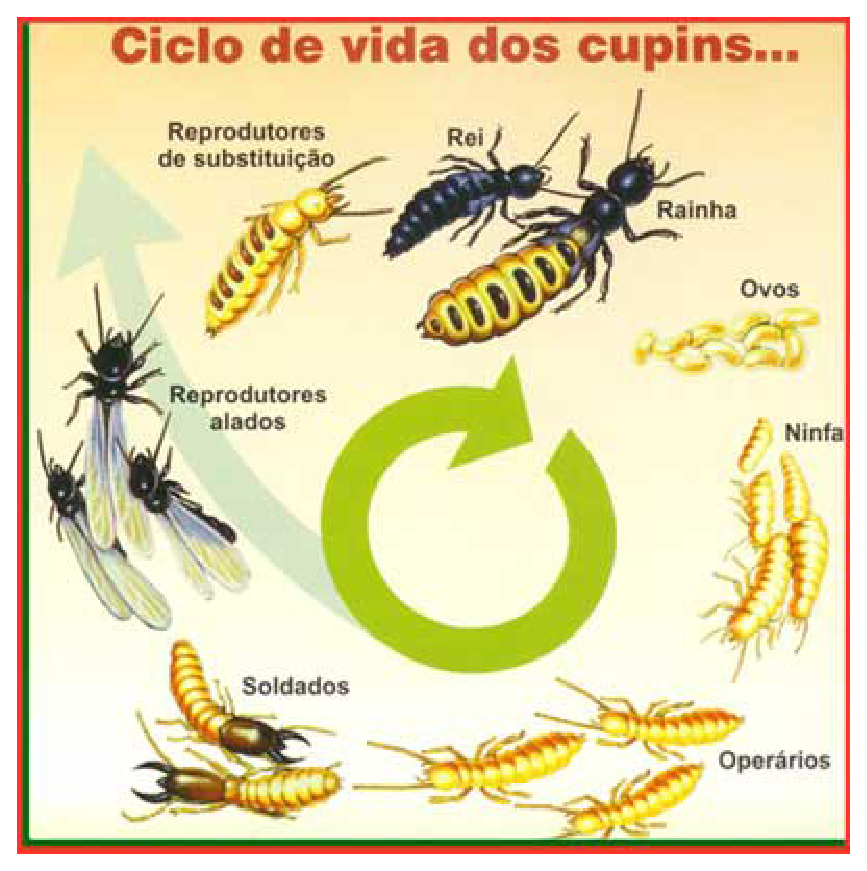
\includegraphics[height=5cm, width=5cm]{ApeA/pragas_ciclo_cupim}
\caption{Uma figura que está no apêndice}\label{FD}
\end{figure}


% Anexos
\annex
\chapter{Exemplo de um Primeiro Anexo} %opcional
% Texto do Primeiro Anexo
\section{Uma Seção do Primeiro Anexo}
% Texto da primeira secao do primeiro anexo
Algum texto na primeira seção do primeiro anexo.



% Glossario
%\itaglossary
%\printglossary

% Folha de Registro do Documento
% Valores dos campos do formulario
\FRDitadata{25 de março de 2015}
\FRDitadocnro{DCTA/ITA/DM-018/2015} %(o número de registro você solicita a biblioteca)
\FRDitaorgaointerno{Instituto Tecnológico de Aeronáutica -- ITA}
%Exemplo no caso de pós-graduação: Instituto Tecnol{\'o}gico de Aeron{\'a}utica -- ITA
\FRDitapalavrasautor{Cupim; Cimento; Estruturas}
\FRDitapalavrasresult{Cupim; Dilema; Construção}
%Exemplo no caso de graduação (TG):
%\FRDitapalavraapresentacao{Trabalho de Graduação, ITA, São José dos Campos, 2015. \NumPenultimaPagina\ páginas.}
%Exemplo no caso de pós-graduação (msc, dsc):
\FRDitapalavraapresentacao{ITA, São José dos Campos. Curso de Mestrado. Programa de Pós-Graduação em Engenharia Aeronáutica e Mecânica. Área de Sistemas Aeroespaciais e Mecatrônica. Orientador: Prof.~Dr. Adalberto Santos Dupont. Coorientadora: Prof$^\textnormal{a}$.~Dr$^\textnormal{a}$. Doralice Serra. Defesa em 05/03/2015. Publicada em 25/03/2015.}
\FRDitaresumo{Aqui começa o resumo do referido trabalho. Não tenho a menor idéia do que colocar aqui. Sendo assim, vou inventar. Lá vai: Este trabalho apresenta uma metodologia de controle de posição das juntas passivas de um manipulador subatuado de uma maneira subótima. O termo subatuado se refere ao fato de que nem todas as juntas ou graus de liberdade do sistema são equipados com atuadores, o que ocorre na prática devido a falhas ou como resultado de projeto. As juntas passivas de manipuladores desse tipo são indiretamente controladas pelo movimento das juntas ativas usando as características de acoplamento da dinâmica de manipuladores. A utilização de redundância de atuação das juntas ativas permite a minimização de alguns critérios, como consumo de energia, por exemplo.
Apesar da estrutura cinemática de manipuladores subatuados ser idêntica a do totalmente atuado, em geral suas caraterísticas dinâmicas diferem devido a presença de juntas passivas. Assim, apresentamos a modelagem dinâmica de um manipulador subatuado e o conceito de índice de acoplamento. Este índice é utilizado na sequência de controle ótimo do \mbox{manipulador}.
A hipótese de que o número de juntas ativas seja maior que o número de
passivas  $(n_{a} > n_{p})$  permite o controle ótimo das juntas passivas, uma vez que na etapa de controle destas há mais entradas (torques nos atuadores das juntas ativas), que elementos a controlar (posição das juntas passivas). }
%  Primeiro Parametro: Nacional ou Internacional -- N/I
%  Segundo parametro: Ostensivo, Reservado, Confidencial ou Secreto -- O/R/C/S
\FRDitaOpcoes{N}{O}
% Cria o formulario
\itaFRD

\end{document}
% Fim do Documento. O massacre acabou!!! :-)
